\documentclass{beamer}

\usepackage[utf8]{inputenc}
\usepackage{fancybox}
\usepackage{environ,verbatim}

\usepackage{tikz}

\newcommand{\ds}{\displaystyle}

\beamertemplatenavigationsymbolsempty

\title{2.3 Linear Equations}

\subtitle{a lecture for MATH F302 Differential Equations}

\author{Ed Bueler, Dept.~of Mathematics and Statistics, UAF}

\date{Fall 2023}


\usetheme{Pittsburgh}


\begin{document}

\setbeamertemplate{itemize item}{$\bullet$}
\setbeamertemplate{itemize subitem}{$\circ$}


\begin{frame}
\titlepage

\centerline{\tiny for textbook: \, D. Zill, \emph{A First Course in Differential Equations with Modeling Applications}, 11th ed.}
\end{frame}


\begin{frame}{linear first-order differential equations}
a \emph{linear} ordinary differential equation has only a first power on both $dy/dx$ and $y$, \emph{and} it can be put in the form
        $$a_1(x) \frac{dy}{dx} + a_0(x) y = g(x)$$
or
        $$\frac{dy}{dx} + P(x) y = g(x)$$

\bigskip
\alert{we can write solutions to such equations in terms of integrals!}
\end{frame}


\begin{frame}{examples}
linear equation standard form: \qquad $\ds \frac{dy}{dx} + P(x) y = g(x)$

\bigskip
Examples:
\begin{itemize}
    \item
        $$\frac{dy}{dx} + y = x+3$$
    Here $P(x)=1$ and $g(x) = x+3$.
    \item
        $$t z' = z + \cos t$$
    which is the same as
        $$\frac{dz}{dt} + \frac{-1}{t} z = \frac{\cos t}{t}$$
    with $P(t) = -1/t$ and $g(t)=\cos t/t$.
\end{itemize}
\end{frame}


\begin{frame}{not an example}
linear equation standard form: \qquad $\ds \frac{dy}{dx} + P(x) y = g(x)$

\bigskip
 \textbf{Not an example:}
 \begin{itemize}
    \item
        $$y \frac{dy}{dx} = x+e^x$$
    this cannot be put in the standard form \dots but it is \emph{separable} (section 2.2)
\end{itemize}
\end{frame}


\begin{frame}{example 1}
before giving general formulas, here's how the method works on an example

\begin{itemize}
    \item \textbf{Example}.
        $$\frac{dy}{dx} + y = x+3$$
\end{itemize}

\vspace{50mm}
\end{frame}


\begin{frame}{solution principle}
to solve a first-order, linear ordinary differential equation $y' + P(x) y = g(x)$ we

 \alert{multiply by a factor which allows us to \emph{undo} the product rule}
\end{frame}


\begin{frame}{recipe}
for $y' + P(x) y = g(x)$ :

\bigskip
\begin{enumerate}
\item find $\mu(x)$ so that $\mu'(x) = P(x) \mu(x)$
\item multiply both sides by $\mu$:
    $$\mu y' + \mu P y = \mu g$$
\item recognize product rule:
    $$(\mu y)' = \mu g$$
\item integrate:
    $$\mu(x) y(x) = \int \mu(x) g(x)\,dx$$
\item solve for $y$:
    $$y(x) = \mu(x)^{-1} \int \mu(x) g(x)\,dx$$
\end{enumerate}
\end{frame}


\begin{frame}{integrating factor}
\noindent \textbf{formula:}  the \alert{integrating factor} $\mu(x)$ is found by
    $$\mu(x) = e^{\int P(x)\,dx}$$
\end{frame}


\begin{frame}{example 2}

\textbf{example:}  \emph{(has an initial condition)}
        $$\frac{dy}{dx} + y = x+3, \qquad y(0)=3$$

\vspace{60mm}
\end{frame}


\begin{frame}
visualization of
        $$\frac{dy}{dx} + y = x+3, \qquad y(0)=3$$

\vspace{10mm}
FIXME %\includegraphics<1>[width=0.8\textwidth]{lineardirfield}

FIXME %\includegraphics<2>[width=0.8\textwidth]{lineardirfieldsoln}
\end{frame}


\begin{frame}
\begin{itemize}
    \item \textbf{Example}.  Newton's law of cooling
        $$\frac{dT}{dt} = k (T_m - T), \qquad T(0)=T_0$$
    where $k,T_m,T_0$ are constants
\end{itemize}

\vspace{5mm}
\hfill FIXME %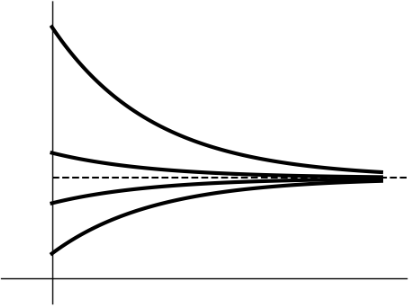
\includegraphics[width=0.8\textwidth]{coolingcurves}
\end{frame}


\begin{comment}
\begin{frame}
\begin{itemize}
    \item \textbf{Example}.  suppose we have a system with solution $s(t)$ which responds to an input $f(t)$:
        $$\dot s = -k s + f(t), \qquad s(0)=0$$
    
    suppose the input is pulses:
\end{itemize}

\vspace{5mm}
FIXME %\includegraphics[width=0.8\textwidth]{pulsetrain}
\end{frame}


\begin{frame}
\begin{itemize}
    \item \textbf{Example}.  
        $$\dot s = -k s + f(t), \qquad s(0)=0$$
    
    the solution is
        $$s(t) = e^{-kt} \int_0^t e^{k\tau} f(\tau)\,d\tau$$
\end{itemize}
\end{frame}
\end{comment}


\begin{frame}
\begin{itemize}
    \item \textbf{Example}.
        $$x^2 y' + x(x+2) y = e^x$$
\end{itemize}
\end{frame}



\begin{frame}{standard expectations}

to learn this material, just listening to a lecture is \emph{not} enough
\begin{itemize}
\item please \emph{read} section 2.2 in the textbook
\item please \emph{do} the Homework for section 2.2
\item search ``separable ODEs'' at YouTube to see more examples
\end{itemize}
\end{frame}

\end{document}

